\documentclass[sigconf]{acmart}

\RequirePackage[l2tabu, orthodox]{nag}

\usepackage[ruled,vlined,linesnumbered]{algorithm2e}
\usepackage[english]{babel}
\usepackage{booktabs}
\usepackage[T1]{fontenc}
\usepackage{graphicx}
\usepackage[utf8]{inputenc}
\usepackage{listings}
\usepackage{url}
\usepackage{xcolor}

% Suppress "multiple pdfs with page group included in a single page" warning
\pdfsuppresswarningpagegroup=1

% Define colors for code highlighting
\definecolor{color-bg}{HTML}{F6F8FA}
\definecolor{color-keyword}{HTML}{D73A49}
\definecolor{color-ident}{HTML}{005CC5}
\definecolor{color-string}{HTML}{032F62}
\definecolor{color-comment}{HTML}{6A737D}

% Listing
\lstset{%
  language={C++},
  basicstyle={\ttfamily},%
  backgroundcolor=\color{color-bg},%
  identifierstyle={\ttfamily},%
  commentstyle={\itshape\color{color-comment}},%
  keywordstyle={\bfseries\color{color-ident}},%
  stringstyle={\ttfamily\color{color-string}},%
  frame={trbl},%
  frameround={tttt},%
  breaklines=true,%
  columns=[l]{fullflexible},%
  numbers=left,%
  numberstyle={\scriptsize},%
  stepnumber=1,%
  numbersep=1em,%
  % lineskip=-0.5ex,%
  mathescape,%
  xleftmargin=2em,%
  framexleftmargin=1.5em,%
}

\begin{document}

% algorithme2
\SetKwFor{PFor}{parallel for}{do}{end}

\acmConference[PEARC '21]{PEARC '21: Practice and Experience in Advanced
Research Computing}{July 18--22, 2021}{Virtual Conference}

\title{kEDM: A Performance-portable Implementation of Empirical Dynamic
Modeling using Kokkos}

\author{Keichi Takahashi}
\email{keichi@is.naist.jp}
\author{Wassapon Watanakeesuntorn}
\email{wassapon.watanakeesuntorn.wq0@is.naist.jp}
\author{Kohei Ichikawa}
\email{ichikawa@is.naist.jp}
\affiliation{%
  \institution{Nara Institute of Science and Technology}
  \city{Nara}
  \country{Japan}
}

\author{George Sugihara}
\email{gsugihara@ucsd.edu}
\affiliation{%
  \institution{University of California San Diego}
  \city{La Jolla}
  \state{California}
  \country{USA}
}

\author{Gerald M. Pao}
\email{pao@salk.edu}
\affiliation{%
  \institution{Salk Institute for Biological Studies}
  \city{La Jolla}
  \state{California}
  \country{USA}
}

\begin{abstract}
    Empirical Dynamic Modeling (EDM) is a state-of-the-art non-linear time
    series analysis framework. Despite its wide applicability, EDM was not
    scalable to large datasets due to its expensive computational cost. To
    overcome this obstacle, researchers have attempted to accelerate EDM from
    both algorithmic and implementational aspects. In our previous work, we
    have developed mpEDM, a massively parallel implementation of EDM targeting
    HPC systems. However, mpEDM maintains different backends for different
    architectures. This design becomes a burden to port to new hardware in the
    current diversifying landscape of HPC systems. In this paper, we design
    and develop kEDM, a performance portable implementation of EDM based on
    the Kokkos performance portability framework. kEDM runs on both CPUs and
    GPUs while based on a single code base. Furthermore, individual kernels
    have been specifically optimized for EDM computation. Benchmarks using
    real-world datasets indicate up to $5.49\times$ speedup compared to mpEDM
    in convergent cross mapping computation.
\end{abstract}

\keywords{Empirical Dynamical Modeling, Performance Portability,
High-Performance Computing}

% https://dl.acm.org/ccs
\begin{CCSXML}
<ccs2012>
   <concept>
       <concept_id>10010147.10010169</concept_id>
       <concept_desc>Computing methodologies~Parallel computing methodologies</concept_desc>
       <concept_significance>500</concept_significance>
       </concept>
   <concept>
       <concept_id>10002944.10011123.10011674</concept_id>
       <concept_desc>General and reference~Performance</concept_desc>
       <concept_significance>300</concept_significance>
       </concept>
 </ccs2012>
\end{CCSXML}

\ccsdesc[500]{Computing methodologies~Parallel computing methodologies}
\ccsdesc[300]{General and reference~Performance}

\maketitle

\section{Introduction}

\begin{figure*}
    \centering
    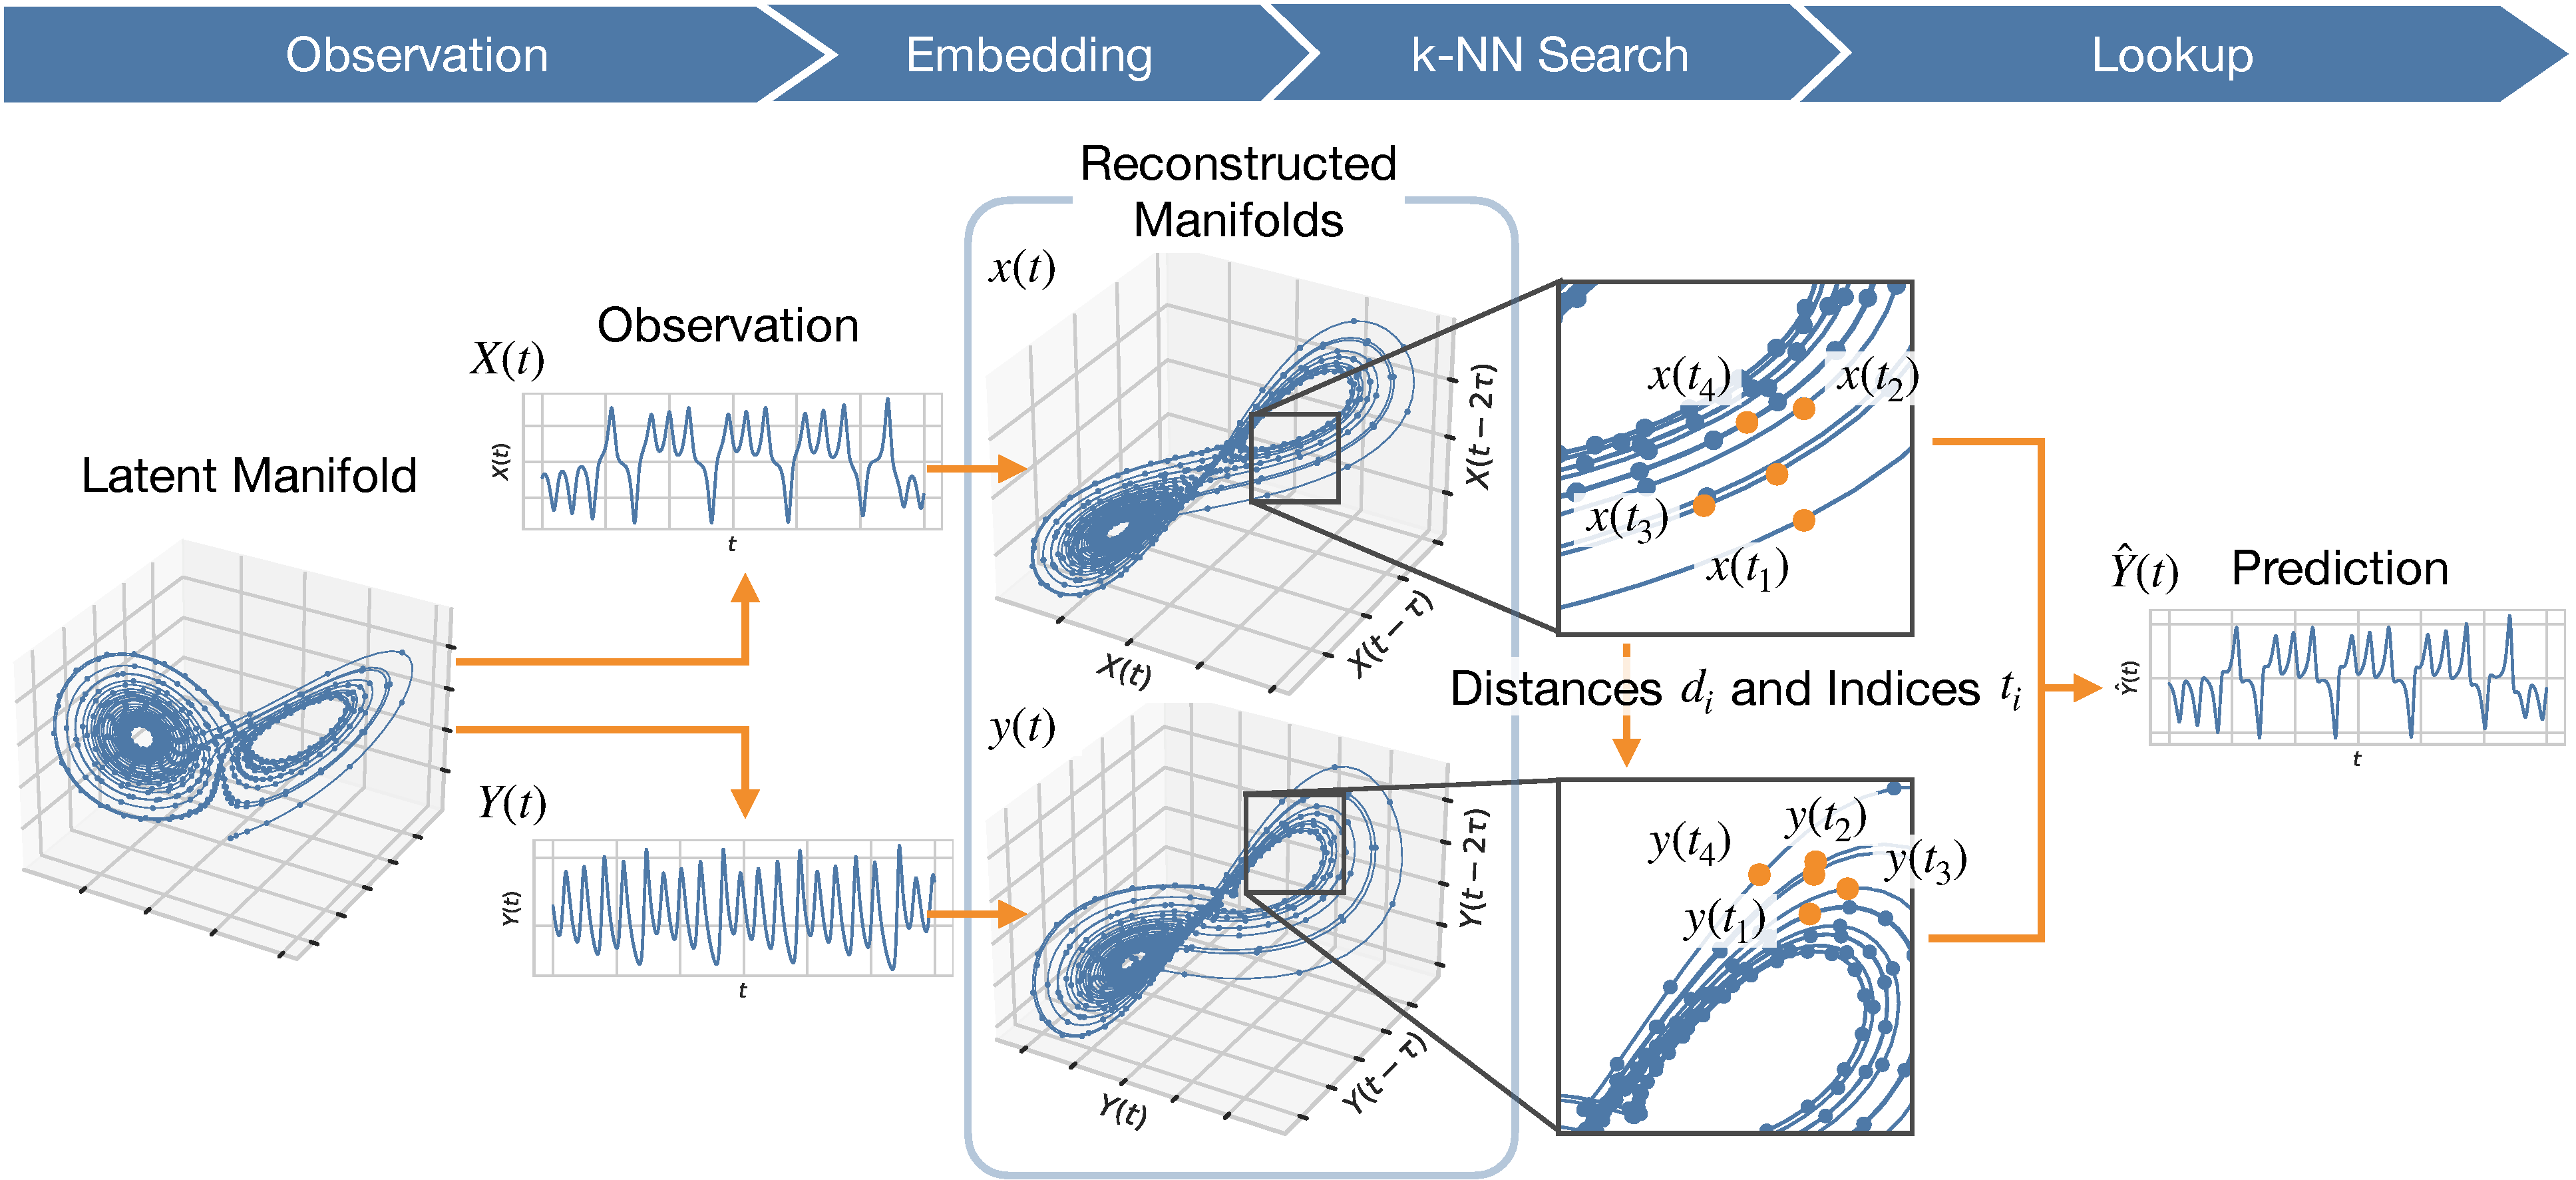
\includegraphics[width=.95\linewidth]{figs/xmap_overview}
    \caption{Overview of Convergent Cross Mapping (CCM)}\label{fig:edm}
\end{figure*}

Empirical Dynamic Modeling (EDM)~\cite{Chang2017} is a state-of-the-art
non-linear time series analysis framework used for various tasks such as
assessing the non-linearity of a system, making short-term forecasts, and
identifying the existence and strength of causal relationships between
variables. Despite its wide applicability, EDM was not scalable to large
datasets due to its expensive computational cost. To overcome this challenge,
researchers have attempted to accelerate EDM from both algorithmic and
implementational aspects~\cite{Pu2019,Ma2014}.

We tackle this challenge by taking advantage of modern HPC systems equipped
with multi-core CPUs and GPUs. We have been developing mpEDM, a massively
parallel distributed implementation of EDM optimized for GPU-centric HPC
systems. In our previous work~\cite{mpedm}, we have deployed mpEDM on the AI
Bridging Cloud Infrastructure (ABCI)\footnote{\url{https://abci.ai/}} to
obtain an all-to-all causal relationship map of all $10^5$ neurons in an
entire larval zebrafish brain. To this date, this is the first causal analysis
of a whole vertebrate brain at single neuron resolution.

Although mpEDM has successfully enabled EDM computation at an unprecedented
scale, there are still challenges remained. The primary challenge is
\textit{performance portability} across diverse hardware platforms. Recent HPC
landscape has seen significant increase in diversity of processors and
accelerators. This is reflected in the design of upcoming exascale HPC systems:
the Frontier system at the Oak Ridge National Laboratory will use AMD EPYC
CPUs and Radeon GPUs while the Aurora system at the Argonne National
Laboratory will employ Intel Xeon CPUs and Xe GPUs. The Fugaku system at RIKEN
uses Fujitsu A64FX Arm CPUs.

The current design of HPC applications has failed to keep up with this trend
of rapidly diversifying HPC systems. Computational kernels of
applications are developed with the native programming model for the
respective hardware (e.g. CUDA on NVIDIA GPUs). mpEDM is no exception and
maintains two completely independent backends for x86\_64 CPUs and NVIDIA
GPUs. However, this design becomes a burden when supporting a diverse set of
hardware platforms because a new backend needs to be developed and maintained
for every platform. Based on this background, various performance portability
frameworks~\cite{Deakin2019, Deakin2020} have been emerged to develop
performance-portable applications from singe code base.

In this paper, we use the Kokkos~\cite{Edwards2014} framework and develop
\textit{kEDM}, a performance-portable implementation of EDM\@ that runs on
both CPUs and GPUs. The new implementation is single-source design and
facilitates the future development and porting to new hardware. Furthermore,
we identify and take advantage of optimization opportunities in mpEDM and
achieve up to 5.5$\times$ higher performance on NVIDIA V100 GPUs.

The rest of this paper is organized as follows. Section~\ref{sec:background}
first introduces EDM briefly and then discusses the challenges in mpEDM\@.
Section~\ref{sec:proposal} presents kEDM, a novel performance-portable
implementation of EDM based on the Kokkos performance portability framework.
Section~\ref{sec:evaluation} compares kEDM and mpEDM using both synthetic and
real-world datasets and assesses the efficiency of kEDM\@.
Section~\ref{sec:conclusion} concludes this paper and discusses future work.

\section{Background}\label{sec:background}

\subsection{Empirical Dynamical Modeling (EDM)}\label{sec:edm}

Empirical Dynamic Modeling (EDM)~\cite{Chang2017} is a non-linear time
series analysis framework based on the Takens' embedding
theorem~\cite{Deyle2011}. Takens' theorem states that given a time-series
observation of a deterministic dynamical system, one can reconstruct the
latent attractor manifold of the dynamical system using time-delayed
embeddings of the observation. While the reconstructed manifold might not
preserve the global structure of the original manifold, it preserves the local
topological features (\textit{i.e.} a diffeomorphism).

Convergent Cross Mapping (CCM)~\cite{Sugihara2012,Natsukawa2017,VanBerkel2020}
is one of the EDM methods that identifies and quantifies the causal
relationship between two time series variables. Figure~\ref{fig:edm} shows the
overview of CCM\@. Given two time series $X(t)$ and $Y(t)$, following four
steps are performed:

\begin{enumerate}
    \item \textit{Embedding}: Time series $X$ and $Y$ are embedded into
        $E$ dimensional state space using their time lags. For example,
        $x$ denotes the embedding of $X$ where $x(t)=(X(t), X(t-\tau),
        \dots, X(t-(E-1) \tau))$. $\tau$ is the time lag. $E$ is
        empirically determined and usually $E<20$ in real-world datasets.
    \item \textit{k-Nearest Neighbor search}: For each point $x(t)$,
         $E+1$ nearest neighbors of $x(t)$ in the state space
        are searched. These neighbors form an $E$ dimensional simplex that
        encloses $x(t)$ in the state space. We refer to the nearest neighbors
        as $x(t_1)$, $x(t_2)$, \dots, $x(t_{E+1})$ and the Euclidean distance
        between $x(t)$ and $x(t_i)$ as $d(t, t_i) =\lVert x(t) - x(t_i)
        \rVert$.
    \item \textit{Lookup}: The prediction $\hat{y}(t)$ for a $y(t)$ is a
        linear combination of points $y(t_1), y(t_2), \dots, y(t_{E+1})$.
        Specifically,
        \begin{equation*}
            \hat{y}(t) = \sum^{E+1}_{i=1} \frac{w_i}{\sum^{E+1}_{i=1}{w_i}} \cdot y(t_i)
        \end{equation*}
        where
        \begin{equation*}
            w_i = \exp\left\{ -\frac{d(t, t_i)}{\min{d(t, t_i)}}\right\}
        \end{equation*}
        The prediction $\hat{Y}(t)$ for $Y(t)$ is made by extracting the first
        component of $\hat{y}(t)$.
    \item \textit{Assessing the prediction}: Pearson's correlation $\rho$
        between $Y$ and $\hat{Y}$ is computed to assess the predictive skill.
        If $\rho$ is high, we conclude that $Y$ ``CCM-causes'' $X$.
\end{enumerate}

These steps are repeated for all pair of time series when performing pairwise
CCM between multiple time series. Out of these steps, $k$-nearest neighbor
search and lookup consume significant runtime and need to optimized. We showed
in our previous work~\cite{mpedm} that one can precompute the nearest
neighbors for every point in $x$ (All $k$-NN search) and store them as lookup
tables of distances and indices. These tables can then be used to make
predictions for all target time series. This approach reduces the number of
$k$-NN search and provides significant speedup.

\subsection{Challenges in mpEDM}\label{sec:challenges}

This subsection discusses the two major challenges in
mpEDM\footnote{\url{https://github.com/keichi/mpEDM}}, our previous
parallel implementation of EDM\@.

\subsubsection{Performance portability across diverse hardware}\label{sec:portability}

The GPU backend of mpEDM was based on ArrayFire~\cite{Malcolm2012}, a general
purpose library for GPU computing. We chose ArrayFire primarily for its
productivity and portability. ArrayFire provides CUDA and OpenCL backends to
run on OpenCL devices. Although it also provides a CPU backend, most of the
functions provided by the CPU backend are neither multi-threaded nor
vectorized. For this reason, we implemented our own implementation for CPUs
using OpenMP\@.

As a result, mpEDM had a ArrayFire-based GPU implementation and a OpenMP-based
CPU implementation of EDM, which doubles the maintenance cost. Considering the
diversifying target hardware, a unified implementation that achieves
consistent and reasonable performance across a diverse set of hardware is
required.

\subsubsection{Kernels optimized for EDM}\label{sec:flexibility}

Since mpEDM was relying on ArrayFire's k-nearest neighbor search function
(\texttt{nearestNeighbour()}), we were unable to modify or tune the k-NN
search to suit our use case and missed opportunities for further optimization.
ArrayFire's nearest neighbor function accepts an array of reference and query
points, and returns a array of closest reference points and their distances
for each query point. This interface is simple and easy-to-use. However, when
applying to EDM, the time-delayed embedding needs to be performed on CPU in
advance and then passed to ArrayFire. This hinders performance because it
increases the amount of data that needs to be copied between the CPU and the
GPU and read from GPU memory.

Another potential optimization opportunity is the partial sort function
\texttt{topk()} invoked in the k-NN search. ArrayFire uses NVIDIA's
CUB\footnote{\url{https://nvlabs.github.io/cub/}} library to implement partial
sort. CUB is a highly optimized library and being used by other libraries such
as Thrust\footnote{\url{https://github.com/NVIDIA/thrust}}. ArrayFire's
\texttt{topk()} function divides the input array into equal sized sub-array
and then calls CUB's parallel radix sort function to sort each sub-array. It
then extracts the top-$k$ elements from each sub-array and concatenates them
into a new array. This is recursively repeated until the global top-$k$
elements are found. Even though this implementation is well-optimized, it may
not be optimal for EDM since the targeted $k$ is relatively small ($\leq 20$).

Finally, we were unable to implement efficient lookups on GPU using ArrayFire.
ArrayFire provides a construct for embarrassingly parallel computation called
\textit{GFOR} that allows one to perform independent for-loops in parallel.
Although we were able to implement lookups using GFOR, the attained
performance was poor. Managing memory consumption and memory copies was also
challenging because ArrayFire implicitly allocates, deallocates and copies
arrays.

\section{kEDM}\label{sec:proposal}

In this section, we first describe the overall design of kEDM followed by a
brief summary of the Kokkos performance portability framework. We then present
the design and implementation of our all $k$-nearest neighbor search and
lookup kernels.

\subsection{Overall Design}

kEDM\footnote{\url{https://github.com/keichi/kEDM}} is our
performance-portable implementation of EDM based on the Kokkos performance
portability framework. To ensure the correctness of the implementation, the
output is validated against the output from mpEDM as well as the reference
implementation pyEDM using automated unit tests.

Prior to implementing kEDM, we have examined a number of popular performance
portability frameworks. These include OpenMP, OpenACC, OpenCL and SYCL\@. We
chose Kokkos  because recent studies~\cite{Martineau2017, Deakin2019, Deakin2020}
have shown that it delivers portable performance on a large set of devices
compared to its alternatives. In addition, it has already been adopted by
multiple production applications~\cite{Sprague2020,Holmen2017,Demeshko2019}.
SYCL and OpenMP are attractive choices as they have grown rapidly over the
last few years in terms of hardware coverage and delivered performance, but we
still consider them immature compared to Kokkos at the point of writing this
paper.

\subsection{Kokkos}

Kokkos~\cite{Edwards2014} is a performance portability framework developed at
the Sandia National Laboratories. The aim of Kokkos is to abstract away the
differences between low-level programming models such as OpenMP, CUDA and HIP
and exposes a high-level C++ interface to the developer. Kokkos allows
developers to build cross-platform and performance-portable applications on a
single source code base.

To parallelize a loop the Kokkos programming model, the developer specifies (1)
the parallel pattern, (2) computational body, and (3) execution policy of the
loop. Available parallel patterns include parallel-for, parallel-reduce and
parallel-scan. The computational body of a loop is given as a lambda function.

The execution policy defines how a loop is executed. For example,
\texttt{RangePolicy} defines a simple 1D range of indices. \texttt{TeamPolicy}
and \texttt{TeamThreadRange} are used to launch teams of threads to exploit
the hierarchical parallelism of the hardware. On a GPU, teams and threads map
to thread blocks and threads within thread blocks, respectively. On a CPU,
teams map to physical cores and threads map to hardware threads within cores.
\texttt{TeamPolicy} gives access to team-private and thread-private scratch
memory, an abstraction of shared memory in GPUs. Each execution policy is
bound to an execution space, an abstraction of where the code runs. The latest
release of Kokkos supports Serial, OpenMP, OpenMP Target, CUDA, HIP, Pthread,
HPX and SYCL\@.

\textit{View} is the fundamental data type in Kokkos and represents a
multidimensional array. Views are explicitly allocated by the user and
deallocated automatically by Kokkos using reference counting. Each view is
associated to a memory space, an abstraction of where the data resides.

Listing~\ref{lst:basic} shows a vector addition  kernel implemented in Kokkos.
In this example, a parallel-for loop is launched that iterates over the 1D
range $1..N$.
Listing~\ref{lst:hierarchical} shows a matrix vector multiplication kernel
using hierarchical parallelism. The outer parallel-for loop launches $M$ teams
that each computes one row of the output vector $y$. The inner parallel-reduce
computes the dot product between one row in $A$ and $x$.

\begin{lstlisting}[caption={Basic data parallel loop},label={lst:basic},float]
Kokkos::parallel_for(RangePolicy<ExecSpace>(N),
KOKKOS_LAMBDA(int i) {
    y(i) = a * x(i) + y(i);
});
\end{lstlisting}

\begin{lstlisting}[caption={Hierarchical data parallel loop},label={lst:hierarchical},float]
parallel_for(TeamPolicy<ExecSpace>(M, AUTO),
KOKKOS_LAMBDA(const member_type &member) {
    int i = member.team_rank();
    float sum = 0.0f;

    parallel_reduce(TeamThreadRange(member, N),
    [=] (int j, float &tmp) {
        tmp += A(i, j) * x(j)
    }, sum);

    single(PerTeam(member),
    [=] () {
        y(i) = sum;
    });
});
\end{lstlisting}

\subsection{All $k$-Nearest Neighbor Search}

We implement the All $k$-NN search using an exhaustive approach similar
to~\cite{Garcia2008,Garcia2010}. That is, we first calculate the pairwise
distances between all embedded library points in the state space and obtain a
pairwise distance matrix. Subsequently, each row of the obtained distance
matrix is partially sorted to find the distances and indices of the points to.

\subsubsection{Pairwise distances}
As discussed in Section~\ref{sec:challenges}, performing the time-delayed
embedding into state space and then calculating the pairwise distances is
inefficient since it increases memory access. Instead, we perform the time
delayed embedding and distance calculation at the same time.

Algorithm~\ref{alg:distances} shows the pairwise distance calculation
algorithm in kEDM\@. Using Kokkos' \texttt{TeamPolicy} and
\texttt{ThreadRange}, we map the outer-most $i$-loop to teams and the $j$-loop to
threads within a team. A consideration on CPU is which loop to vectorize.
Since the inner-most $k$-loop is short ($E \leq 20$) in our use case,
vectorizing it is not profitable. We therefore use \textit{SIMD types}
\footnote{\url{https://github.com/Kokkos/simd-math}} to vectorize the
$j$-loop. SIMD types are short vector with overloaded operators that map to
intrinsic functions. SIMD types are mapped to scalars on GPUs and do not
impose any overhead. Note that the library time series is reused if $E > 1$
and we can expect more reuse with larger $E$. In addition, we explicitly cache
$\mathrm{library} (k \tau + i)$ (where $k=1 \dots E$) on team-local scratch
memory to speed up memory access.

\begin{algorithm}
    \SetAlgoLined
    \DontPrintSemicolon
    \KwIn{Library time series $x$ of length $L$, embedding dimension $E$, time lag $\tau$}
    \KwOut{Pairwise distance matrix $D$ ($L \times L$)}
    \tcp{\texttt{TeamPolicy}}
    \PFor{$i \leftarrow 1$ \KwTo $L$}{
        \tcp{\texttt{ThreadRange}}
        \PFor{$j \leftarrow 1$ \KwTo $L$}{
            $D(i, j) \leftarrow 0$\;
            \For{$k \leftarrow 1$ \KwTo $E$}{
                $D(i, j) \leftarrow D(i, j) + (x(k \tau + i) - x(k \tau + j))^2$\;
            }
        }
    }
    \caption{Pairwise distances}%
    \label{alg:distances}
\end{algorithm}

\subsubsection{Top-$k$ search}

The top-$k$ kernel is challenging to implement in a performance-portable manner
because state-of-the-art top-$k$ algorithms~\cite{Johnson2019,Shanbhag2018}
are usually optimized for specific hardware. For this reason, we designed and
implemented a top-$k$ search algorithm that works on both CPU and GPU
efficiently.

Algorithm~\ref{alg:partial-sort} shows the algorithm. In our algorithm, each
thread team finds the top-$k$ elements from one row of the distance matrix a
time. Each thread within a thread team maintains a local priority queue on
scratch memory that holds the top-$k$ elements it has seen so far. Each thread
reads the distance matrix in a coalesced manner and pushes the element to its
local queue. Once this is finished, one leader thread in each thread team merges
the local queues within the team and writes the final top-$k$ elements to
memory.

% We also tried to fuse the pairwise distance kernel and top-$k$ kernel into one
% kernel but could not gain any speedup.

% \begin{figure}
    % \centering
    % 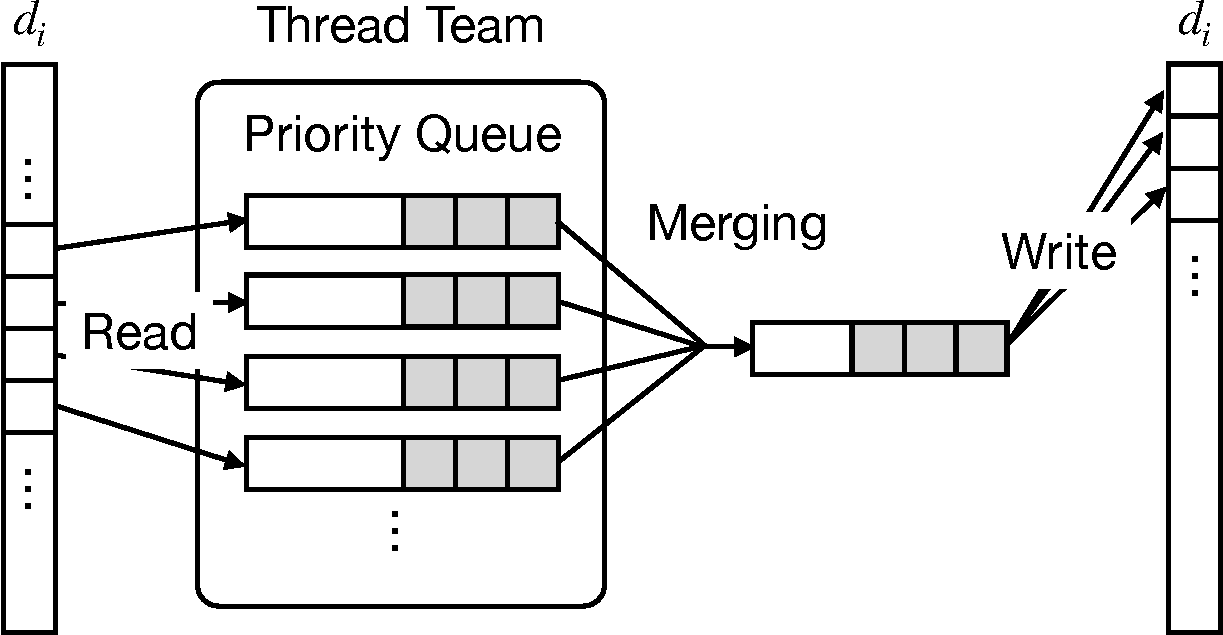
\includegraphics[width=.8\columnwidth]{figs/sorting}
    % \caption{Top-$k$ sorting algorithm}%
    % \label{fig:topk}
% \end{figure}

\begin{algorithm}
    \SetAlgoLined
    \DontPrintSemicolon
    \KwIn{Pairwise distance matrix $D$}
    \KwOut{Top-$k$ distance matrix $D'$}
    \tcp{\texttt{TeamPolicy}}
    \PFor{$i \leftarrow 1$ \KwTo $L$}{
        \tcp{\texttt{ThreadRange}}
        \PFor{$j \leftarrow 1$ \KwTo $L$}{
            Insert $D(i, j)$ into local priority queue\;
        }
        \For{$j \leftarrow 1$ \KwTo $k$}{
            \For{$j \leftarrow 1$ \KwTo \# of threads}{
                $D'(i, j) \leftarrow$ Pop element from priority queue\;
            }
        }
    }
    \caption{Partial sort}%
    \label{alg:partial-sort}
\end{algorithm}

\subsection{Lookup}

Given a library and a target time series, suppose the optimal embedding
dimension of the target time series is $E$. We use the $E$-dimensional embedding
of the library to predict the target. To maximize reuse of the lookup table, we
can group the target time series by its optimal embedding dimension.

Algorithm~\ref{alg:lookup} shows the lookup routine. The outer most $i$-loop
iterates over all time series of which optimal embedding dimension is $E$ and
parallelized using \texttt{TeamPolicy}. Each team performs prediction of one
target time series. The $j$-loop is parallelized using \texttt{TeamThreadRange}
and makes predictions of each time point within a time series (line 5). The
inner most serial $k$-loop is unrolled to exploit ILP\@. Since Kokkos currently
provide a feature to indicate loop unrolling, we use the \texttt{\#pragma
unroll} directive here. The loop body requires indirect access to the target
time series using the indices table. To speed up random access, we cache the
target time series in team-private scratch memory.

In case the raw predictions are not needed and only the assessment of predictive
skill is needed, kEDM does not write out the predicted time series to global
memory. Instead, Pearson’s correlation is computed on-the-fly. Kokkos’ custom
reduction feature is used to implement parallel calculation of correlation
coefficient. The algorithm is based on a numerically stable algorithm for
computing (co-)variance proposed in~\cite{Schubert2018}.

\begin{algorithm}
    \SetAlgoLined
    \DontPrintSemicolon
    \KwIn{Target time series $y$, top-$k$ distance matrix $D_k$, top-$k$ index
    matrix $T_k$, embedding dimension $E$}
    \KwOut{Predicted time series $\hat{y}$}
    \PFor{$i \leftarrow 1$ \KwTo $N$}{
        \PFor{$j \leftarrow 1$ \KwTo $L$}{
            \For{$k \leftarrow 1$ \KwTo $E+1$}{
                $\hat{y}(i, j) \leftarrow \hat{y}(i, j) + D(j, k) \cdot y(T(j, k))$ \;
            }
        }
    }
    \caption{Lookup}%
    \label{alg:lookup}
\end{algorithm}

\section{Evaluation}\label{sec:evaluation}

In this section we compare kEDM with mpEDM using micro benchmarks and
real-world datasets. Furthermore, we conduct a roofline analysis of kEDM to
assess the efficiency of our implementation.

\subsection{Evaluation Environment}

% use table?

We evaluated kEDM on two compute servers installed at the Salk Institute: (1)
Ika and (2) Aori. Ika is equipped with two sockets of 20-core Intel Xeon Gold
6148 CPUs, one NVIDIA V100 PCIe card and 376 GiB of RAM\@. Aori is equipped with
two sockets of 64-core AMD EPYC 7742 CPUs and 1 TiB of RAM\@. kEDM was built
with Kokkos 3.2 on both machines. On Aori, we used the AMD Optimizing C/C++
Compiler (AOCC) 2.2.0, a fork of Clang by AMD. On Ika, we used the NVIDIA CUDA
Compiler (NVCC) 10.1.

\subsection{Micro benchmarks}

We implemented micro benchmarks to measure the performance of the individual
kernels we described in Section~\ref{sec:proposal} and compare them with
mpEDM\@.

Figure~\ref{fig:breakdown-knn-v100} shows the runtime of the All k-NN search
of kEDM and mpEDM on NVIDIA V100. The result indicates that the pairwise
distance calculation in kEDM is significantly faster than mpEDM (up to
6.6$\times$). This is because the embedding is done during the distance
calculation on the GPU\@. The partial sort is also faster if $E$ is small. If
$E=1$, kEDM is 6.2$\times$ faster than mpEDM\@. However, kEDM's performance
degrades as $E$ increases and slightly underperforms mpEDM when $E=20$.
Another issue is warp divergence.

Figure~\ref{fig:breakdown-knn-epyc} shows the runtime of the All k-NN search
on AMD EPYC 7742. It should be noted that the partial sort algorithm in mpEDM
uses a max heap to store the elements. Since the $E$ we are interested is
small, the difference between linear time and logarithmic time is not visible.

% lower occupancy due to the thread local queues

Figures~\ref{fig:breakdown-lookup-v100} and~\ref{fig:breakdown-lookup-epyc}
show the runtime of the lookup on V100 and EPYC 7742, respectively. The runtime
excludes cross correlation calculation. Note that we ran kEDM only on
V100 since mpEDM lacks a lookup kernel for GPU as described earlier in
Section~\ref{sec:flexibility}. As we can see from the plots, kEDM on V100
consistently outperforms EPYC 7742 by a factor of 3$\times$ to 4$\times$.
Interestingly, kEDM slightly outperforms mpEDM on EPYC. One of the reasons could
be that we load the target time series to scratch memory before performing
lookups. Even though CPUs do not have user-managable memory, accessing the
target time series might have loaded the time series on cache and improved the
cache hit ratio.

\begin{figure}
    \centering
    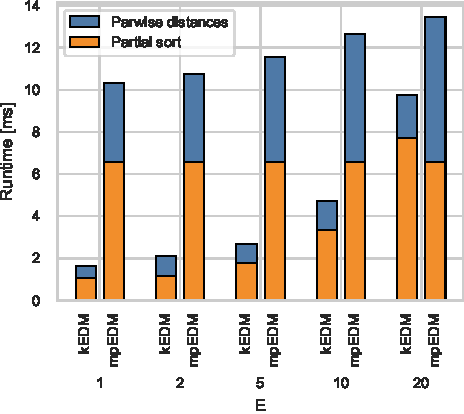
\includegraphics{figs/breakdown_knn_v100}
    \caption{Breakdown of All k-NN search runtime on V100 ($L=10^4$)}%
    \label{fig:breakdown-knn-v100}
\end{figure}

\begin{figure}
    \centering
    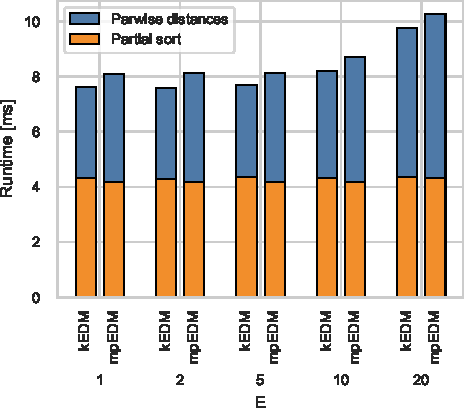
\includegraphics{figs/breakdown_knn_epyc}
    \caption{Breakdown of All k-NN search runtime on EPYC 7742 ($L=10^4$)}%
    \label{fig:breakdown-knn-epyc}
\end{figure}

\begin{figure}
    \centering
    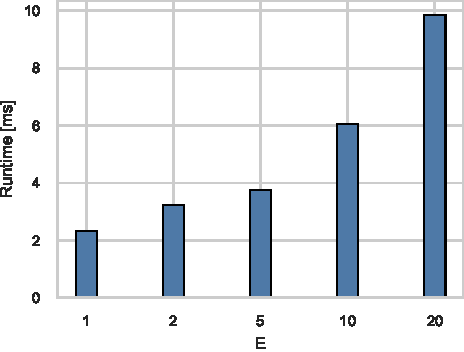
\includegraphics{figs/runtime_lookup_v100}
    \caption{Runtime of lookups on V100 ($L=10^4, N=10^5$)}%
    \label{fig:breakdown-lookup-v100}
\end{figure}

\begin{figure}
    \centering
    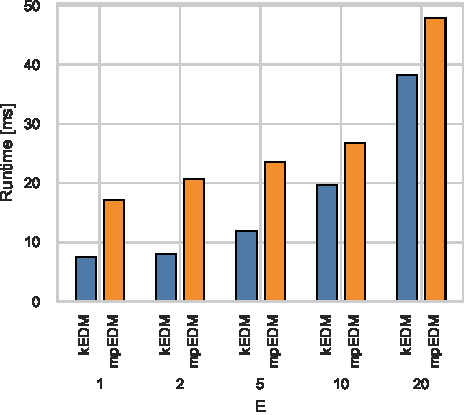
\includegraphics{figs/runtime_lookup_epyc}
    \caption{Runtime of lookups on EPYC 7742 ($L=10^4, N=10^5$)}%
    \label{fig:breakdown-lookup-epyc}
\end{figure}

\subsection{Real-world datasets}

We used several real-world datasets with diverse number and length of time
series that reflect the variety of use cases.
% Need short description of the datasets and acknowledge their authors
Table~\ref{tbl:real-world} shows the runtime for performing a pairwise CCM for
each dataset. The results demonstrate that kEDM outperforms mpEDM in most
cases. In particular, kEDM shows significantly better (up to 5.5$\times$)
performance than mpEDM on an Ika\@. This is because kEDM performs the lookups
on the GPU instead of the CPU\@.

\begin{table*}
\centering
\caption{Benchmark results using real-world datasets}%
\label{tbl:real-world}
\begin{tabular}{@{}lrrrrrrrr@{}}
\toprule
             & \multicolumn{1}{c}{} & \multicolumn{1}{c}{} & \multicolumn{3}{c}{V100 \& Xeon Gold 6148 } & \multicolumn{3}{c}{EPYC 7742} \\ \cmidrule(l){4-6}  \cmidrule(l){7-9}
Dataset      & \multicolumn{1}{c}{\# of Time Series} & \multicolumn{1}{c}{\# of Time Steps} & kEDM & mpEDM & Speedup & kEDM & mpEDM & Speedup \\ \midrule
Fish1\_Normo &  154    & 1,600  &      3s &     11s & 3.67$\times$ &      3s &      4s & 1.33$\times$ \\
Fly80XY      &  82     & 10,608 &     11s &     50s & 4.55$\times$ &     22s &     30s & 1.36$\times$ \\
Genes\_MEF   &  45,318 & 96     &    344s &    334s & 0.97$\times$ &     96s &    139s & 1.45$\times$ \\
Subject6     &  92,538 & 3,780  &  5,391s & 29,579s & 5.49$\times$ & 12,145s & 11,571s & 0.95$\times$ \\
Subject11    & 101,729 & 8,528  & 20,517s & 85,217s & 4.15$\times$ & 43,812s & 38,542s & 0.88$\times$ \\
F1           &  8,520  & 29,484 & 11,372s & 20,128s & 1.77$\times$ & 23,001s & 19,950s & 0.87$\times$ \\ \bottomrule
\end{tabular}
\end{table*}

\subsection{Efficiency}

To assess the efficiency of our implementation, we conducted a roofline
analysis~\cite{Williams2008} of our kernels. The compute and memory ceilings
on each platform were measured using the Empirical Roofline Toolkit (ERT)\footnote{\url{https://bitbucket.org/berkeleylab/cs-roofline-toolkit/}} 1.1.0.
Since ERT fails to measure the L1 cache bandwidth on GPUs, we used the
theoretical peak performance instead. We followed the methodology presented
in~\cite{Yang2020a,Yang2020b} to measure the arithmetic intensity and the
attained FLOP/s. Nvprof 10.1 and likwid~\cite{Treibig2010} 5.0.1 were used to
collect the required metrics on GPU and CPU, respectively.
We used an artificial dataset containing $10^5$ time series each having $10^4$
time series. This scale reflects our largest use case.

% 1.38*80*32*4/1024 = 13.8 TiB/s
% (frequency)*(# of SMs)*(bank size)*(bank width)
% memory alignment issue and vectorized loads/stores

Figures \ref{fig:roofline-distances-v100} and \ref{fig:roofline-distances-epyc}
show the hierarchical roofline models for the pairwise distance kernel on V100
and EPYC 7742, respectively. As expected, the arithmetic intensity of the
pairwise distance kernel increased with the embedding dimension since the
reuse of the time series improves. On V100, the kernel was bounded by HBM
bandwidth when $E=1$. However, the kernel was not able to reach the rooflines
as $E$ increases. We found using NVIDIA Nsight profiler that the load store
units were saturated because of excessive many memory transactions. A common
technique to reduce the number of memory transactions is to use vectorized
loads and stores; however, it is not applicable here because the memory
alignment depends on the user-supplied parameters $E$ and $\tau$. On EPYC 7742,
the kernel is clearly hitting the L3 cache roofline.

\begin{figure}
    \centering
    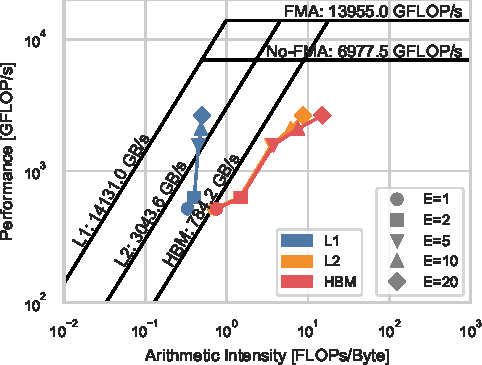
\includegraphics{figs/roofline_distances_v100}
    \caption{Roofline analysis of pairwise distance kernel on V100 ($L=10^4$)}%
    \label{fig:roofline-distances-v100}
\end{figure}

\begin{figure}
    \centering
    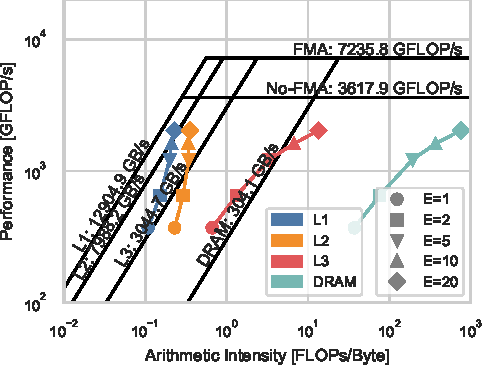
\includegraphics{figs/roofline_distances_epyc}
    \caption{Roofline analysis of pairwise distance kernel on EPYC 7742 ($L=10^4$)}%
    \label{fig:roofline-distances-epyc}
\end{figure}

Figures \ref{fig:roofline-lookup-v100} and \ref{fig:roofline-lookup-eypc} show
the rooflines for the lookup kernel on V100 and EPYC 7742, respectively. These
plots indicate that the lookup kernel is bounded by the L2 cache on V100 and
the L1 cache on EPYC 7742. This is explained from the fact that the distance
and index matrix fit on the respective caches. For example, the footprint of
the distance and index matrix is 1.6 MB if $E=20$. This fits on EPYC 7742's L1
cache (4 MiB) and V100's L2 cache (6 MiB).

\begin{figure}
    \centering
    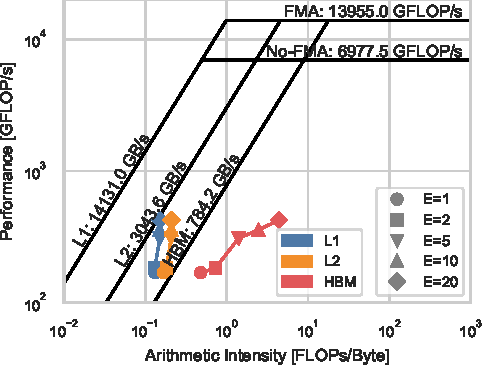
\includegraphics{figs/roofline_lookup_wo_rho_v100}
    \caption{Roofline analysis of lookup kernel on V100 ($L=10^4, N=10^5$)}%
    \label{fig:roofline-lookup-v100}
\end{figure}

\begin{figure}
    \centering
    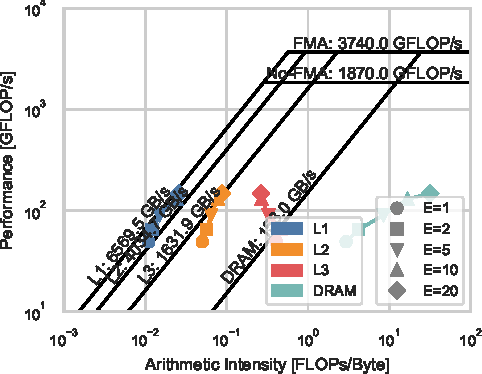
\includegraphics{figs/roofline_lookup_wo_rho_epyc}
    \caption{Roofline analysis of lookup kernel on EPYC 7742 ($L=10^4, N=10^5$)}%
    \label{fig:roofline-lookup-eypc}
\end{figure}

\section{Conclusion \& Future Work}\label{sec:conclusion}

We designed and developed kEDM, a performance portable implementation of EDM
based on the Kokkos performance portability framework. The new implementation
is single-source and runs on both CPUs and GPUs. Furthermore, several
inefficiencies have been removed from mpEDM and kernels have been custom
tailored. Benchmarks using real-world datasets indicate up to $5.49\times$
speedup in convergent cross mapping computation.

In the future, we will implement a Python binding to facilitate adoption by
users. We will also evaluate on other hardware platforms such as AMD GPUs and
Fujitsu A64FX ARM processors.

\begin{acks}
This work was supported by JSPS KAKENHI Grant Number JP20K19808 (KT) and an
Innovation grant by the Kavli Institute for Brain and Mind (GMP).
\end{acks}

% check consistency (especially month)
\bibliographystyle{IEEEtran}
\bibliography{references}

\end{document}
